\documentclass[12pt]{article}

\usepackage[margin=0.5in]{geometry}

\usepackage{hyperref}
\hypersetup{
    colorlinks=true,
    linkcolor=blue,
    filecolor=magenta,      
    urlcolor=blue,
}
 
\urlstyle{same}

\usepackage{datetime}
\newdateformat{specialdate}{\twodigit{\THEDAY}.\twodigit{\THEMONTH}.\THEYEAR}

\usepackage{polski}
\usepackage[polish]{babel}
\usepackage[utf8]{inputenc}

\usepackage{titling}

\usepackage{framed}
\usepackage[svgnames]{xcolor}
\colorlet{shadecolor}{Gainsboro!50}

\usepackage{float}
\usepackage{graphicx}
\graphicspath{ {./images/} }

\usepackage{verbatim}

\usepackage{caption}
\captionsetup[figure]{name=Fig.}

\title{Lab Gene Family Trees}
\author{Maciej Sikora}
\date{\specialdate\today}


\begin{document}
\maketitle

\section{Wstępne statystyki i wizualizacje drzew}

\begin{figure}[H]
\begin{center}
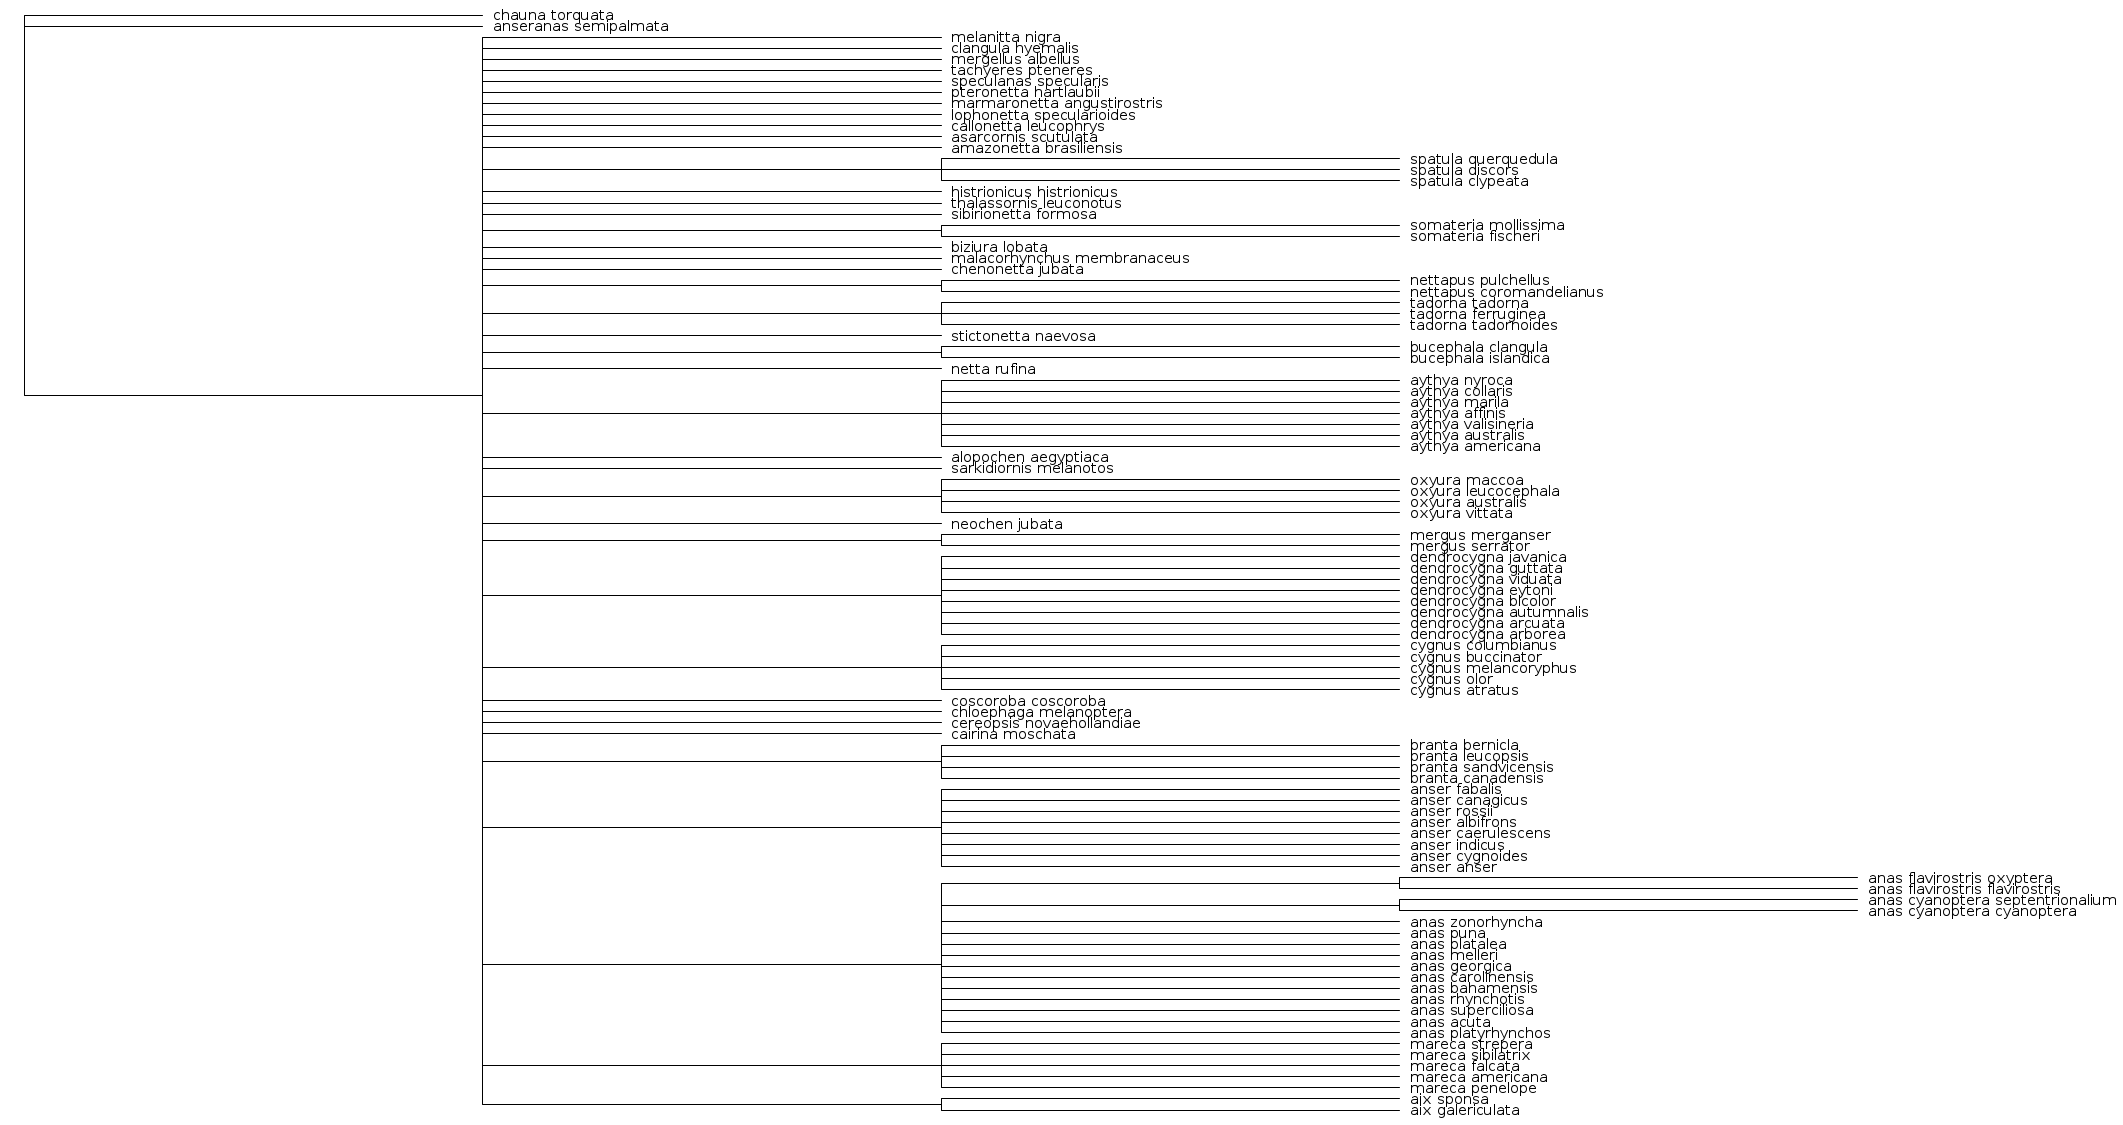
\includegraphics[width=\textwidth]{taxonomy}
\caption{Drzewo taxonomiczne}
\end{center}
\end{figure}

\begin{figure}[H]
\begin{center}
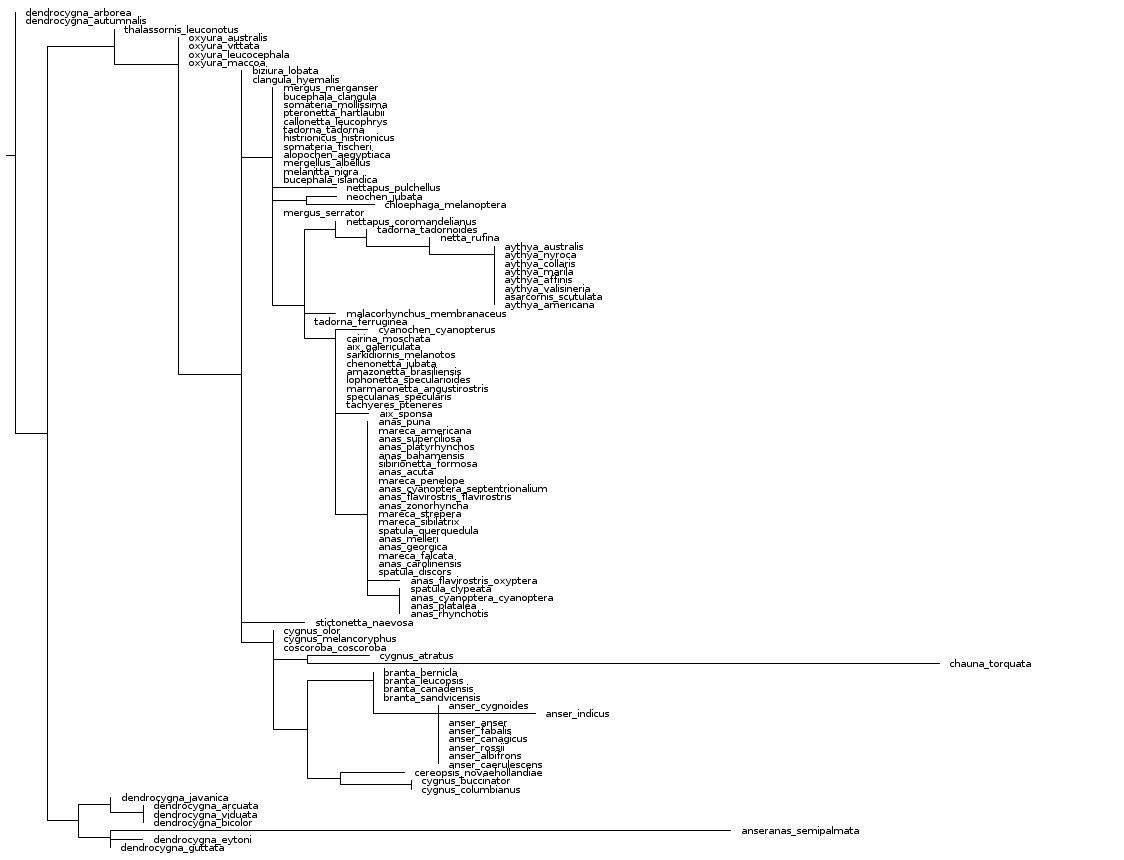
\includegraphics[width=\textwidth]{ml}
\caption{Drzewo maximum likelihood}
\end{center}
\end{figure}

\begin{figure}[H]
\begin{center}
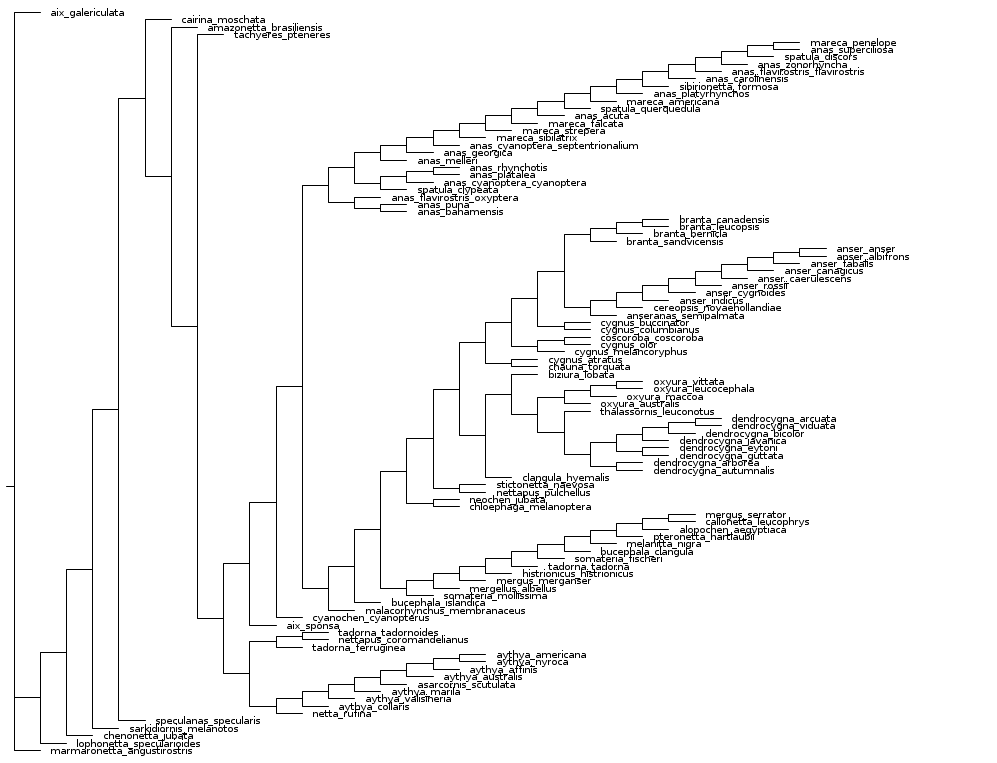
\includegraphics[width=\textwidth]{mp}
\caption{Drzewo maximum parsimony}
\end{center}
\end{figure}

\begin{figure}[H]
\begin{center}
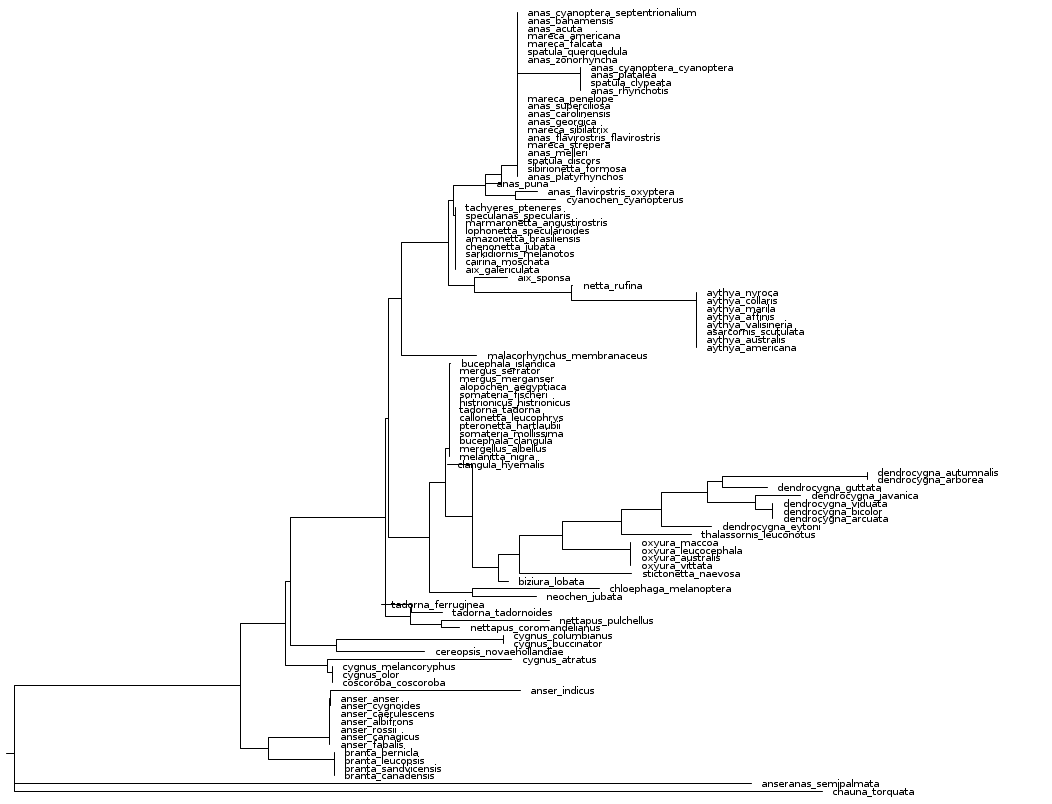
\includegraphics[width=\textwidth]{nj}
\caption{Drzewo neighbor joining}
\end{center}
\end{figure}

Odległości Robinsona Fouldsa dla drzew:
\begin{itemize}
\item ML vs MP: 164
\item ML vs NJ: 174
\item MP vs NJ: 158
\end{itemize}

\section{Porównanie z drzewem gatunków}
\begin{itemize}
\item ''Anas'' występuje w otoczeniu ''Mareca'' dla wszyskich drzew
\item ''Anser'' obok ''Branta'' dla wszystkich drzew
\item ''Dendrocygna'' występuje obok ''Cygnus'' na drzewie gatunków, ale nie u pozostałych
\item ''Tadoma'' występuje obok ''Nettapus'' na drzewie gatunków, ale nie u pozostałych
\item Gatunki są zwykle zgrupowane
\end{itemize}


\end{document}

\begin{comment}
BEGIN EXAMPLE PARAGRAPH:

-----Kod w szarym boxie-----
\begin{shaded}\small
\begin{alltt}
KOD
\end{alltt}
\end{shaded}

-----Wstawianie obrazka-----
\begin{figure}[H]
\begin{center}
\includegraphics[width=\textwidth]{raw_url_fasta}
\caption{Przykład umiejscowienia sekwencji przy użyciu surowego linku.}
\end{center}
\end{figure}

-----Tabela-----
\begin{center}
\begin{tabular}{ | l | l | } 
\hline
Nazwa & Dodatek do linku\\ 
\hline
\hline
AC & id\\
\hline
Entry name & entry\%20name\\ 
\hline
Czy Reviewed & reviewed\\ 
\hline
Referencje do Pfam & database(Pfam)\\ 
\hline
Sekwencja & sequence\\ 
\hline
\end{tabular}
\end{center}

\end{comment}